\chapter{Cônicas}

A fórmula da distância entre dois pontos é muitas vezes usada para achar a equação de uma curva cuja definição geométrica depende de uma ou mais distâncias. Um das curvas mais simples desta espécie é a circunferência, mas outras curvas como parábolas, elipses e hipérboles também estão relacionadas a distâncias entre elementos geométricos (pontos, retas).

\section{Parábola}
Curva do plano formada pelos pontos equidistantes de um ponto fixo $F$ (foco) e de uma reta $d$ (diretriz). Ou seja, um ponto $P(x, y)$ pertence à parábola, se e somente se, $$d(P, F)=d(P, d)$$

Uma parábola possui os seguintes elementos:
\begin{itemize}
  \item \textbf{foco:} é o ponto $F$.
  \item \textbf{diretriz:} é a reta $d$.
  \item \textbf{eixo:} é a reta que passa por $F$ e é perpendicular a $d$. Observe que toda parábola é simétrica em relação ao seu eixo.
  \item \textbf{vértice:} é o ponto V de interseção da parábola com o seu eixo.
\end{itemize}

Para este texto, chamaremos a distância entre o foco $F$ e a reta diretriz $d$ por parâmetro da parábola e será dado por: $p=d(F, d)$. Observe que a distância entre o vértice e a reta diretriz, e o vértice e o foco são metade deste valor, ou seja $\displaystyle d(V, d)=d(V, F)= \frac{p}{2}$.

\subsection{Parábola com eixo vertical}

Inicialmente vamos considerar a parábola com eixo vertical, ou seja, o eixo é paralelo ao eixo $Oy$. Mais particularmente, consideremos o próprio eixo $Oy$ como eixo da parábola, e o vértice sendo $V(0, 0)$.

Neste caso, o foco F será um ponto sobre o eixo $Oy$, e possuirá coordenadas $\displaystyle F(0, \frac{p}{2})$. A reta diretriz será dada pela equação $y=-\frac{p}{2}$.

A parábola será dada pelos pontos $P(x, y)$, de modo que\footnote{Observe que ponto da projeção de $P$ sobre $d$ será dado por $P'(x,-\frac{p}{2})$.}:
\begin{eqnarray*}
d(P, F) & = & d(P, d)   \\
d(P, F) & = & d(P, P')   \\
\sqrt{(x-0)^2+\left(y-\frac{p}{2}\right) ^2} & = & \sqrt{(x-x)^2+\left(y+\frac{p}{2}\right)^2}  \\
x^2+\left(y-\frac{p}{2}\right)^2 & = & 0^2+\left(y+\frac{p}{2}\right)^2  \\
x^2+y^2-py+\frac{p^2}{4} & = & y^2+py+\frac{p^2}{4} \\
x^2 & = & 2py 
\end{eqnarray*}

Ou seja, a equação reduzida da parábola com vértice $V(0, 0)$, foco $\displaystyle F(0,\frac{p}{2})$ e diretriz $\displaystyle y=-\frac{p}{2}$ será dada por: $$x^2=2py$$

\begin{figure}[H]
\centering
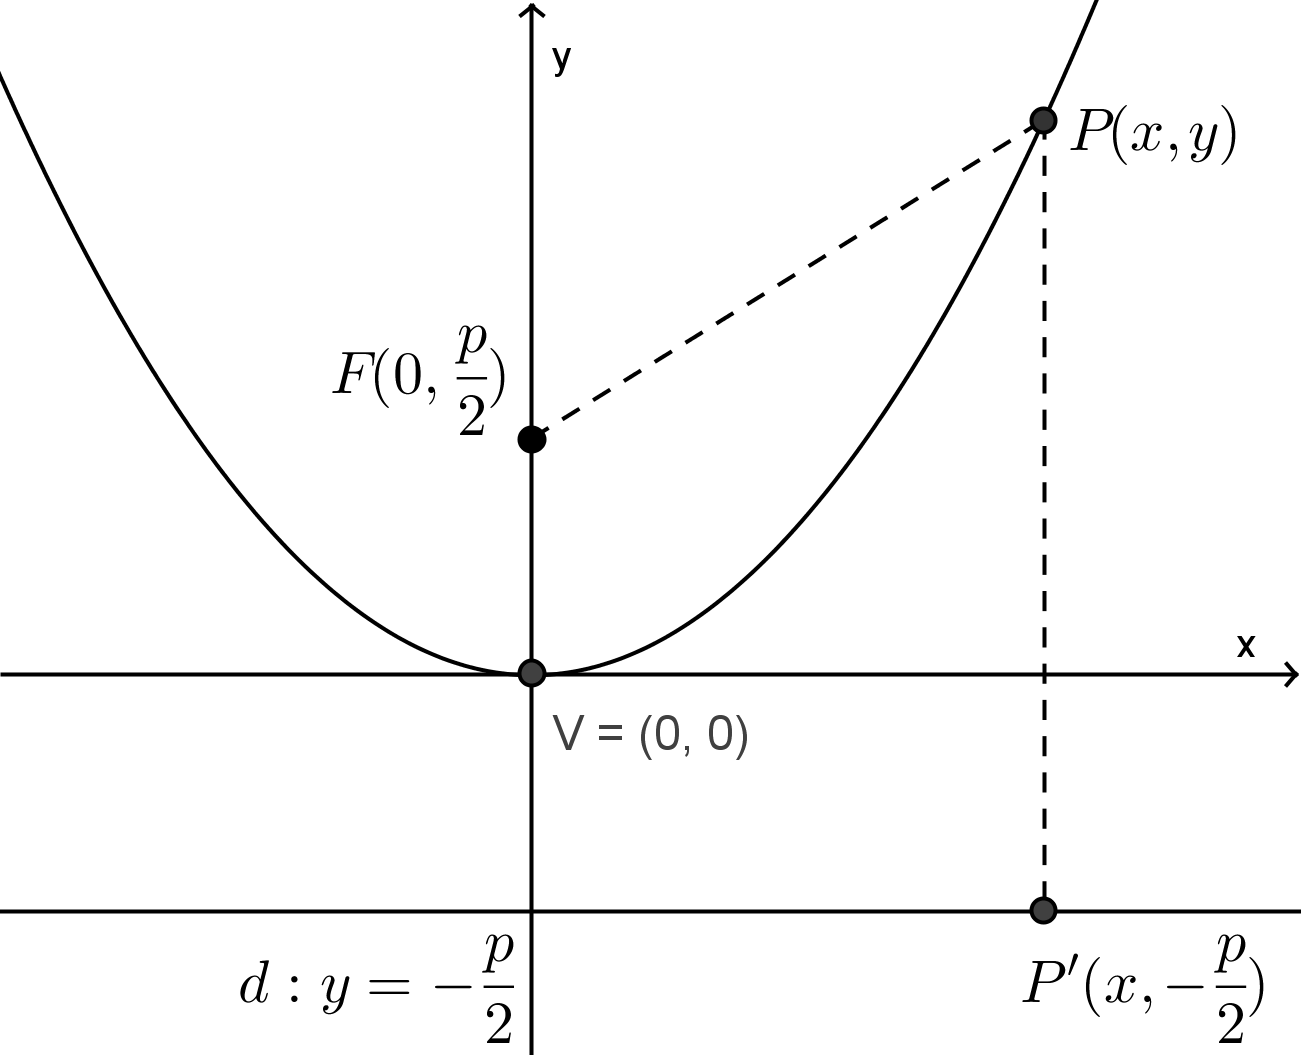
\includegraphics[width=0.4\linewidth]{analitica/imagens/parabolav1.png}
\caption{Parábola com eixo $Oy$}
\label{fig:para1}
\end{figure}

Observe que:
\begin{itemize}
  \item $p>0$: concavidade (abertura) da parábola para cima.
  \item $p<0$: concavidade (abertura) da parábola para baixo.
\end{itemize}

Mais genericamente, se considerarmos como eixo da parábola, qualquer reta vertical paralela a $Oy$, considerando o vértice $V(h, k)$, teremos a equação: $$(x-h)^2=2p(y-k)$$

%\begin{multicols}{2}

\begin{exemplo} Obtenha a equação da parábola com vértice $V(-1, 2)$, eixo paralelo ao eixo $Oy$, e que $d(F, V)=1$.

Primeiramente devemos observar que $d(F, V)=\frac{p}{2}$, e portanto:
\begin{eqnarray*}
\frac{p}{2} & = & d(F, V)   \\
\frac{p}{2} & = & 1   \\
p & = & 2
\end{eqnarray*}

Como a equação é paralela ao eixo $Oy$, então sua equação é da forma:
\begin{eqnarray*}
(x-h)^2&=&2p(y-k)  \\
(x+1)^2&=&4(y-2)
\end{eqnarray*}


\begin{figure}[H]
\centering
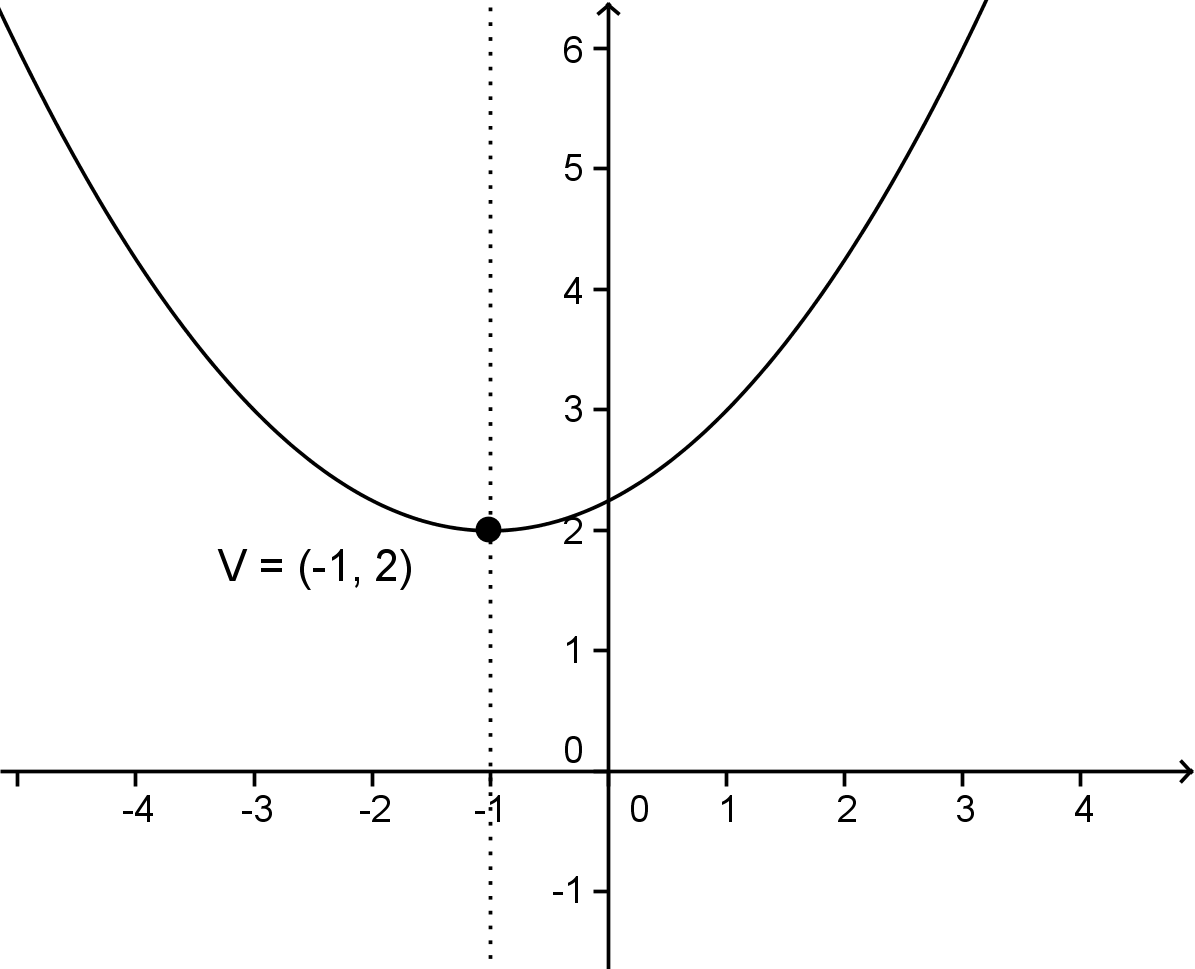
\includegraphics[width=0.4\linewidth]{analitica/imagens/exemplo1.png}
%\caption{Circunferência}
\label{fig:exe1}
\end{figure}

A equação acima ainda pode receber a forma chamada de \textit{equação geral}
\begin{eqnarray*}
(x+1)^2&=&4(y-2) \\
x^2+2x+1&=&4y-8 \\
x^2+2x-4y+9&=&0
\end{eqnarray*}


Se isolarmos o $y$, temos a forma chamada de \textit{equação explícita}
\begin{eqnarray*}
0&=&x^2+2x-4y+9 \\
4y&=&x^2+2x+9 \\
y&=&\frac{x^2}{4}+\frac{x}{2}+\frac{9}{4}
\end{eqnarray*}


\end{exemplo}
%\end{multicols}


\subsection{Parábola com eixo horizontal}

Agora, vamos considerar a parábola com eixo horizontal, ou seja, o eixo é paralelo ao eixo $Ox$. Mais particularmente, consideremos o próprio eixo $Ox$ como eixo da parábola, e o vértice sendo $V(0, 0)$. Neste caso, o foco F será um ponto sobre o eixo $Ox$, e possuirá coordenadas $\displaystyle F\left(\frac{p}{2}, 0\right)$. A reta diretriz será dada pela equação $\displaystyle x=-\frac{p}{2}$.

A parábola será dada pelos pontos $P(x, y)$, de modo que\footnote{Observe que ponto da projeção de $P$ sobre $d$ será dado por $P'(-\frac{p}{2},y)$.}:

\begin{eqnarray*}
d(P, F) & = & d(P, d)   \\
d(P, F) & = & d(P, P')   \\
\sqrt{\left(x-\frac{p}{2}\right)^2+(y-0)^2} & = & \sqrt{\left(x+\frac{p}{2}\right)^2+(y-y)^2}  \\
\left(x-\frac{p}{2}\right)^2+y^2 & = & \left(x+\frac{p}{2}\right)^2+0^2  \\
x^2-px+\frac{p^2}{4}+y^2 & = & x^2+px+\frac{p^2}{4}   \\
y^2 & = & 2px 
\end{eqnarray*}

Ou seja, a equação reduzida da parábola com vértice $V(0, 0)$, foco $F(\frac{p}{2},0)$ e diretriz $\displaystyle x=-\frac{p}{2}$ será dada por: $$y^2=2px$$

\begin{figure}[H]
\centering
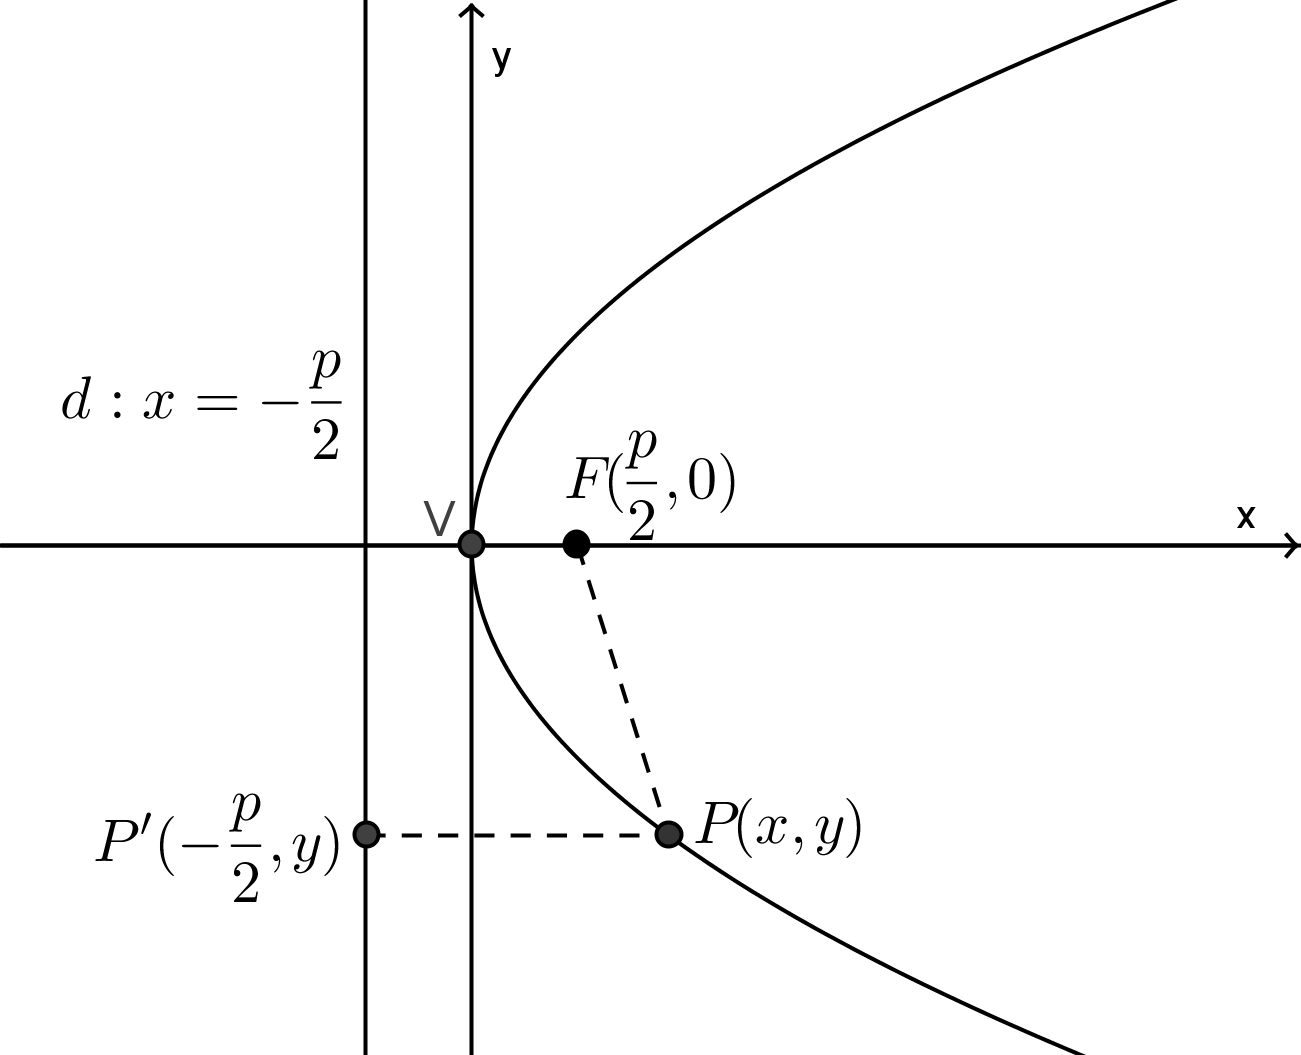
\includegraphics[width=0.5\linewidth]{analitica/imagens/parabolah1.png}
\caption{Parábola com eixo $Ox$}
\label{fig:parah1}
\end{figure}

Observe que:
\begin{itemize}
  \item $p>0$: concavidade (abertura) da parábola para direita.
  \item $p<0$: concavidade (abertura) da parábola para esquerda.
\end{itemize}

Mais genericamente, se considerarmos como eixo da parábola, qualquer reta horizontal paralela a $Ox$, considerando o vértice $V(h, k)$, teremos a equação: $$(y-k)^2=2p(x-h)$$

\section{Circunferência}

A circunferência pode ser definida como o conjunto de todos os pontos que equidistam de um ponto fixo $C$. O ponto fixo é chamado centro da circunferência e a distância de qualquer de seus pontos ao centro é o raio dessa circunferência. Se o centro é o ponto $C(a, b)$ e o raio é o número positivo $r$, e se $P(x, y)$ é um ponto qualquer da circunferência, então a definição acima se traduz

\begin{multicols}{2}
\begin{figure}[H]
\centering
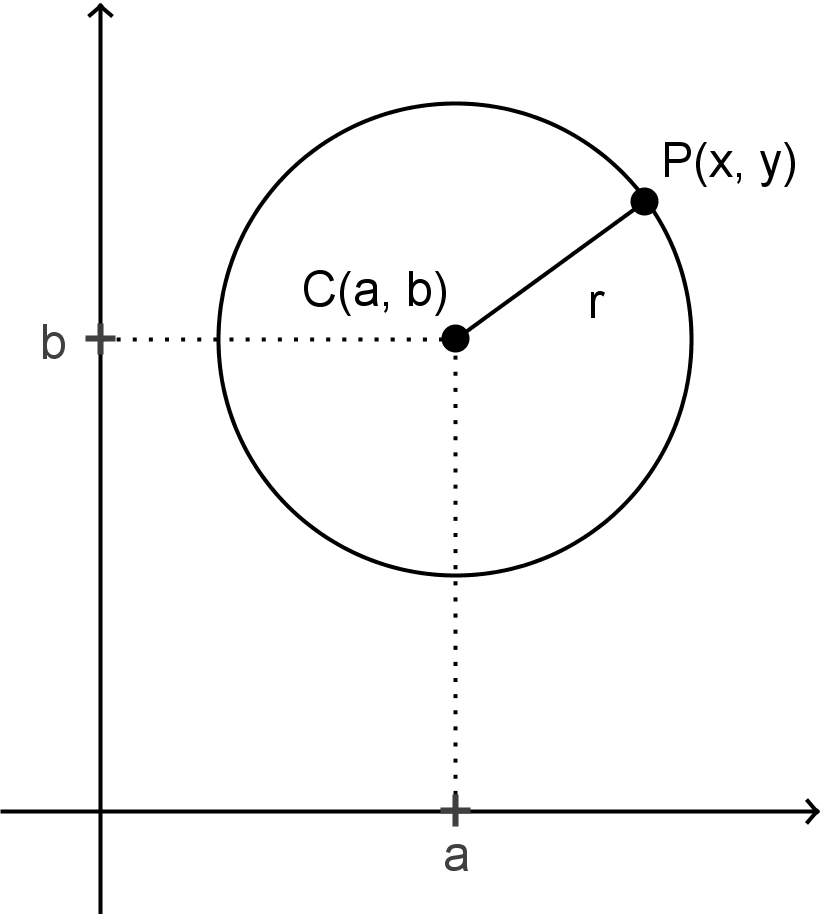
\includegraphics[width=0.45\linewidth]{analitica/imagens/circ1.png}
\caption{Circunferência}
\label{fig:circ1}
\end{figure}

\begin{eqnarray*}
d(P, C) & = & r   \\
\sqrt{(x-a)^2+(y-b)^2} & = & r  \\
(x-a)^2+(y-b)^2 & = & r^2
\end{eqnarray*}
\end{multicols}


Ou seja, a circunferência de centro $C(a, b)$ e raio $r$ é dada por $$(x-a)^2+(y-b)^2= r^2$$

\section{Elipse}

Elipse é o conjunto de todos os pontos de um plano cuja soma das distâncias a dois pontos fixos $F_1$ e $F_2$ desse plano é constante.

Consideremos no plano dois pontos distintos $F_1$ e $F_2$, tal que a distância $d(F_1, F_2)=2c$, e um número real positivo $a$, de modo que $a>c$.

Seja $P(x, y)$ um ponto do plano, $P$ pertence à elipse se, e somente se,

$$d(P, F_1)+d(P, F_2)=2a$$


\begin{figure}[H]
\centering
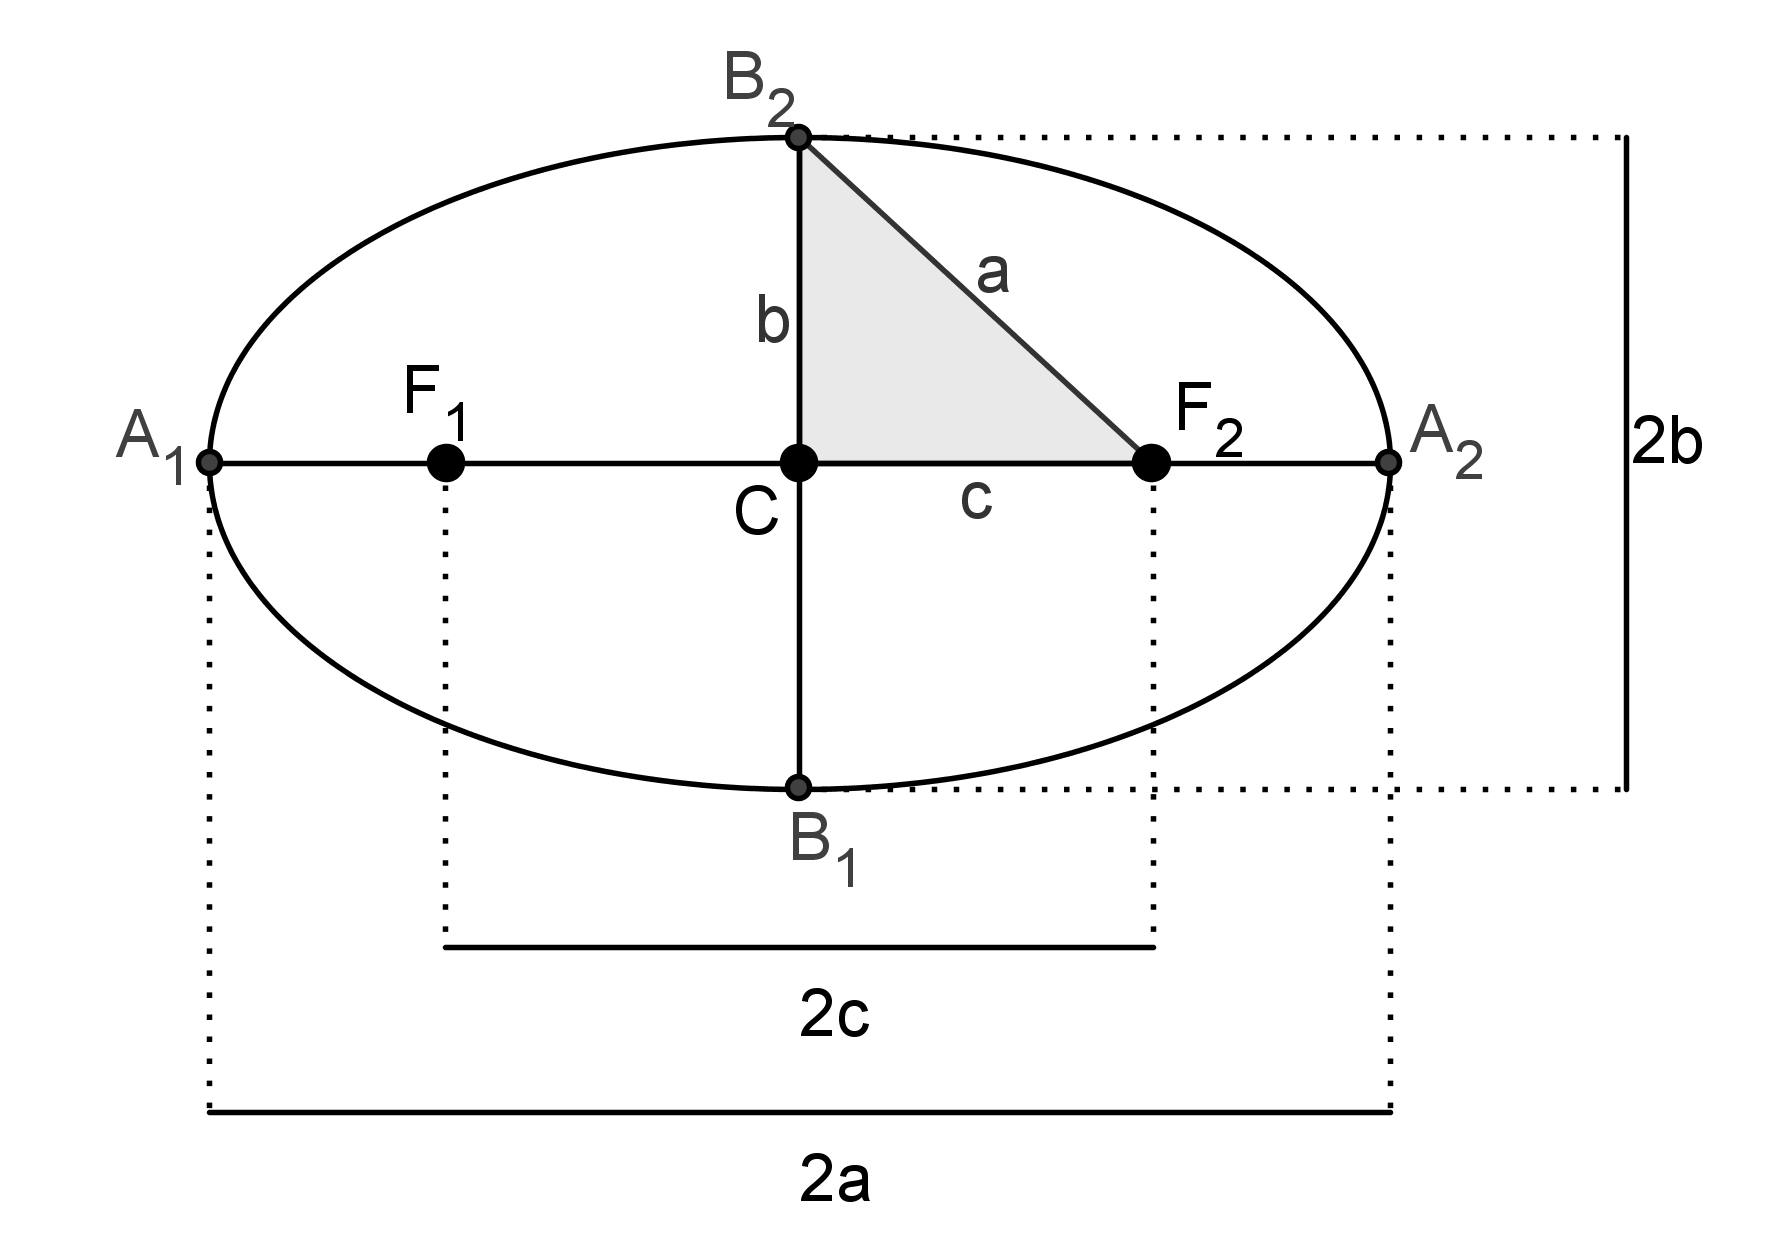
\includegraphics[width=0.45\linewidth]{analitica/imagens/elipse.png}
\caption{Elementos da Elipse}
\label{fig:elipse}
\end{figure}

A elipse possui os seguintes elementos:
\begin{itemize}
  \item \textbf{Focos:} são os pontos $F_1$ e $F_2$.
  \item \textbf{Distância focal:} é a distância $2c$ entre os focos.
  \item \textbf{Centro:} é o ponto médio do segmento $F_1F_2$.
  \item \textbf{Eixo Maior:} é o segmento $A_1A_2$ de comprimento $2a$. O eixo maior é o segmento que contém os focos.
  \item \textbf{Eixo Menor:} é o segmento $B_1B_2$ de comprimento $2b$. O eixo menor é perpendicular ao segmento $A_1A_2$ no centro $C$.
  \item \textbf{Excentricidade:} é o número real $\displaystyle e=\frac{c}{a}$. Indica o ``grau de achatamento'' da elipse. Excentricidade perto de 0 indicam elipses quase circulares, enquanto que excentricidade perto de 1 indica elipse bastante achatada ou alongada.
\end{itemize}

Observe que: $$a^2=b^2+c^2$$ e esta igualdade mostra que $b$ e $c$ são menores do que $a$.

\subsection{Equações reduzidas da elipse}

Considere um sistema cartesiano, e adotemos os focos da elipse sobre o eixo $Ox$. Desta forma, use $F_1(c, 0)$, $F_2(-c,0)$, a distância entre os focos $2c$, a constante da definição $2a$ e utilize a fórmula da distância para deduzir a equação reduzida da elipse.
\begin{eqnarray*}
d(P, F_1)+d(P, F_2)&=&2a \\
\sqrt{(x+c)^2+y^2} + \sqrt{(x-c)^2+y^2}& = & 2a  \\
&\vdots &\\
(a^2-c^2)x^2+a^2y^2&=&a^2b^2 \\
b^2x^2+a^2y^2&=&a^2b^2 \\
\frac{x^2}{a^2}+\frac{y^2}{b^2}& =& 1
\end{eqnarray*}
que é a \textit{equação reduzida} para esta situação.

\begin{figure}[H]
\centering
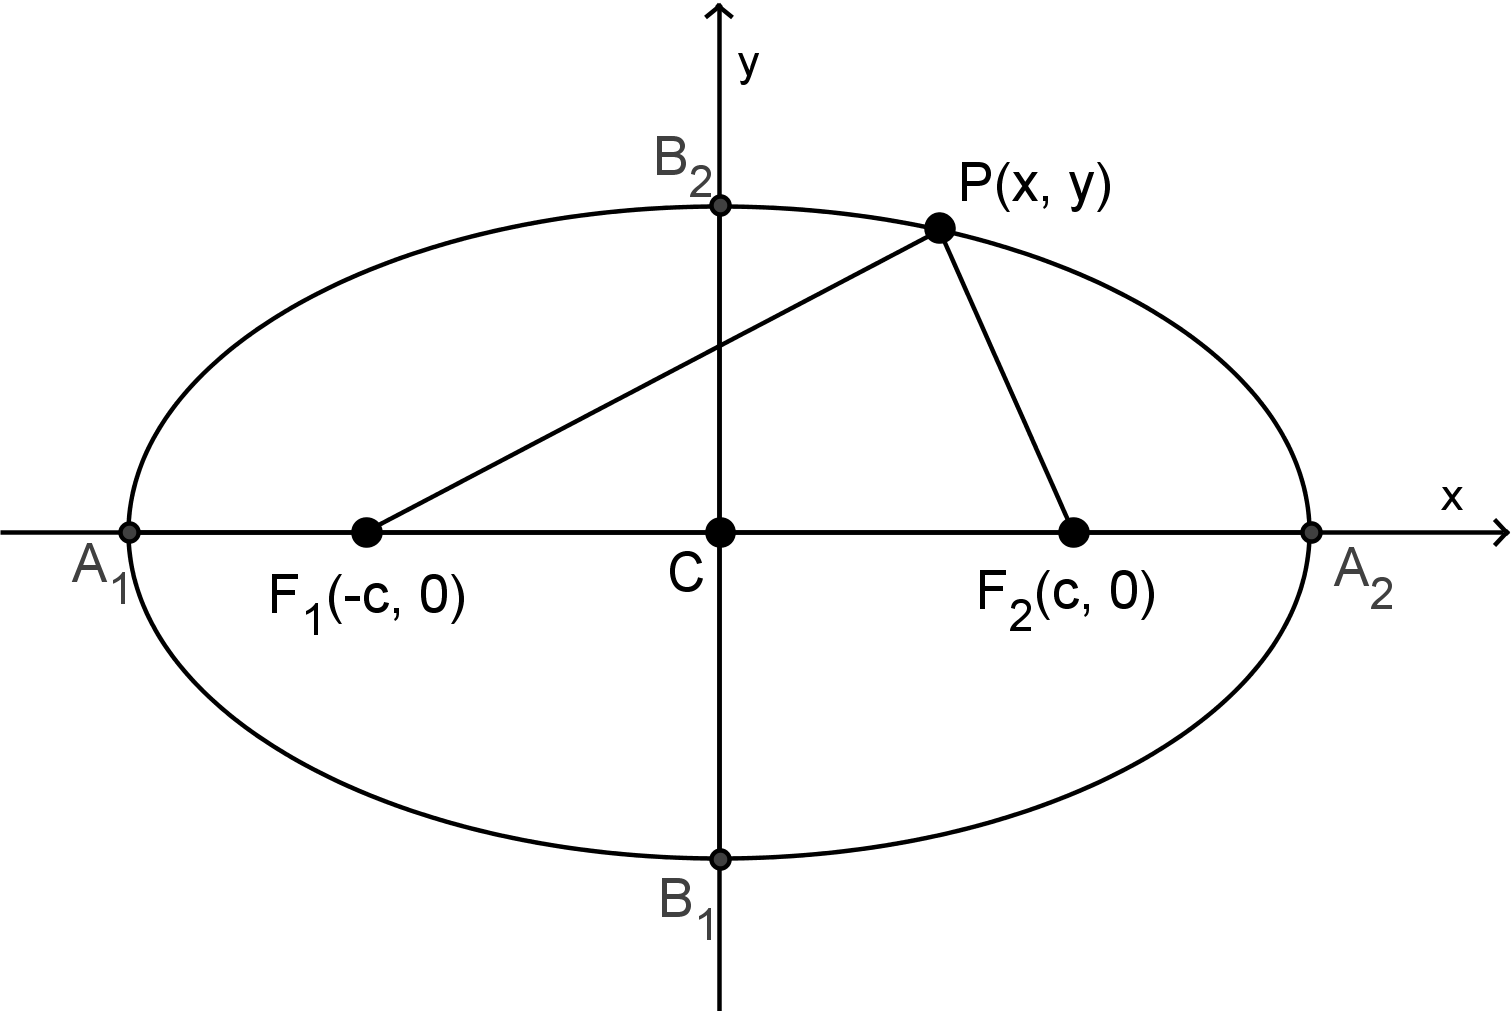
\includegraphics[width=0.45\linewidth]{analitica/imagens/elipseh1.png}
\caption{Elipse }
\label{fig:elipseh1}
\end{figure}

Para o caso do eixo maior sobre o eixo $Oy$, teremos uma situação análoga, com a seguinte \textit{equação reduzida}:

$$\frac{x^2}{b^2}+\frac{y^2}{a^2}=1$$

Para identificar o eixo maior da elipse, basta verificar onde está o maior denominador. Por exemplo, para a elipse $\displaystyle \frac{x^2}{16}+\frac{y^2}{9}=1$, temos que o eixo maior será $Ox$, pois o termo $x^2$ possui o maior denominador.

Para um caso mais geral, considerando o centro da elipse em $C(h, k)$, a equação da elipse será dada por $$\frac{\left(x-h\right)^2}{a^2}+\frac{\left(y-k\right)^2}{b^2}=1$$ que possui o eixo maior paralelo a $Ox$, ou $$\frac{\left(x-h\right)^2}{b^2}+\frac{\left(y-k\right)^2}{a^2}=1$$ que possui eixo maior paralelo ao eixo $Oy$.

\section{Hipérbole}

Hipérbole é o conjunto de todos os pontos de um plano cuja diferença das distâncias a dois pontos fixos $F_1$ e $F_2$ desse plano é constante.

Consideremos no plano dois pontos distintos $F_1$ e $F_2$, tal que a distância $d(F_1, F_2)=2c$, e um número real positivo $a$, de modo que $a<c$.

Seja $P(x, y)$ um ponto do plano, $P$ pertence à hipérbole se, e somente se,

$$|d(P, F_1)-d(P, F_2)|=2a$$

Ou, seja, a hipérbole é uma curva com dois ramos, e desta forma um ponto $P$ pertence à hipérbole se, e somente se
$$d(P, F_1)-d(P, F_2)=\pm 2a$$

\begin{figure}[H]
\begin{minipage}[b]{0.45\linewidth}
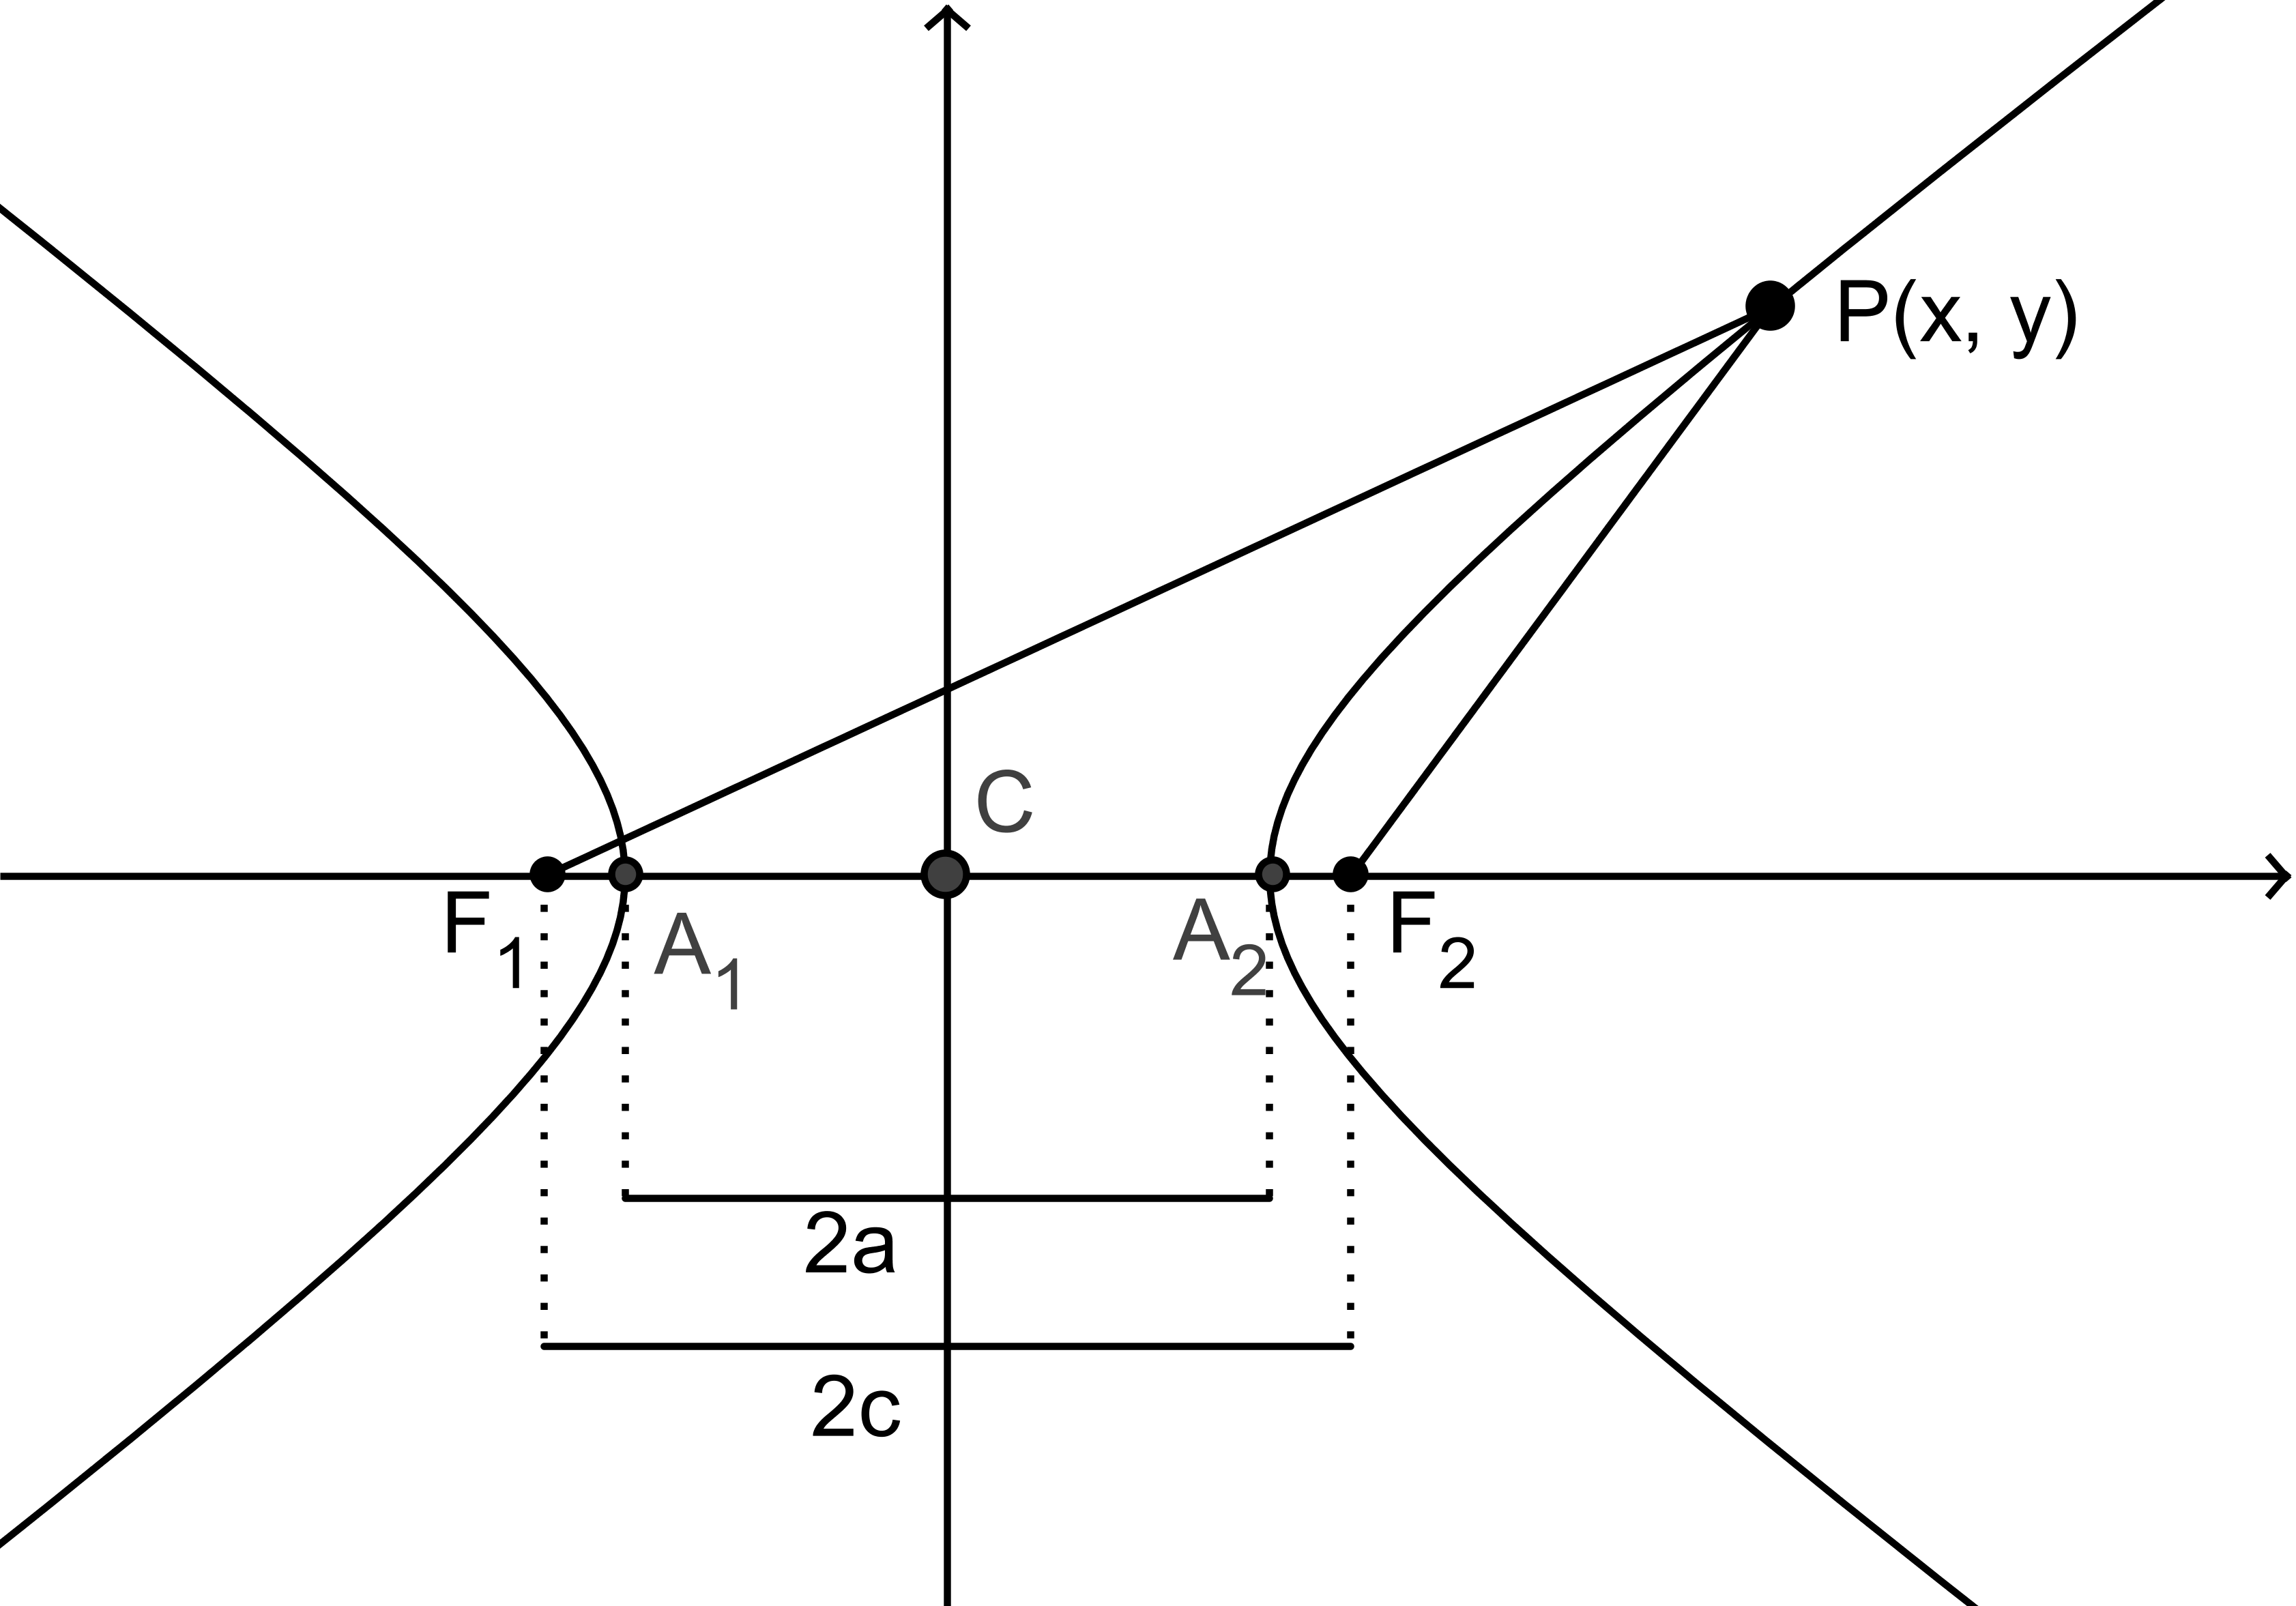
\includegraphics[width=\linewidth]{analitica/imagens/hiperboleh.png}
\caption{Hipérbole}
\label{fig:hiperboel}
\end{minipage} \hfill
\begin{minipage}[b]{0.45\linewidth}
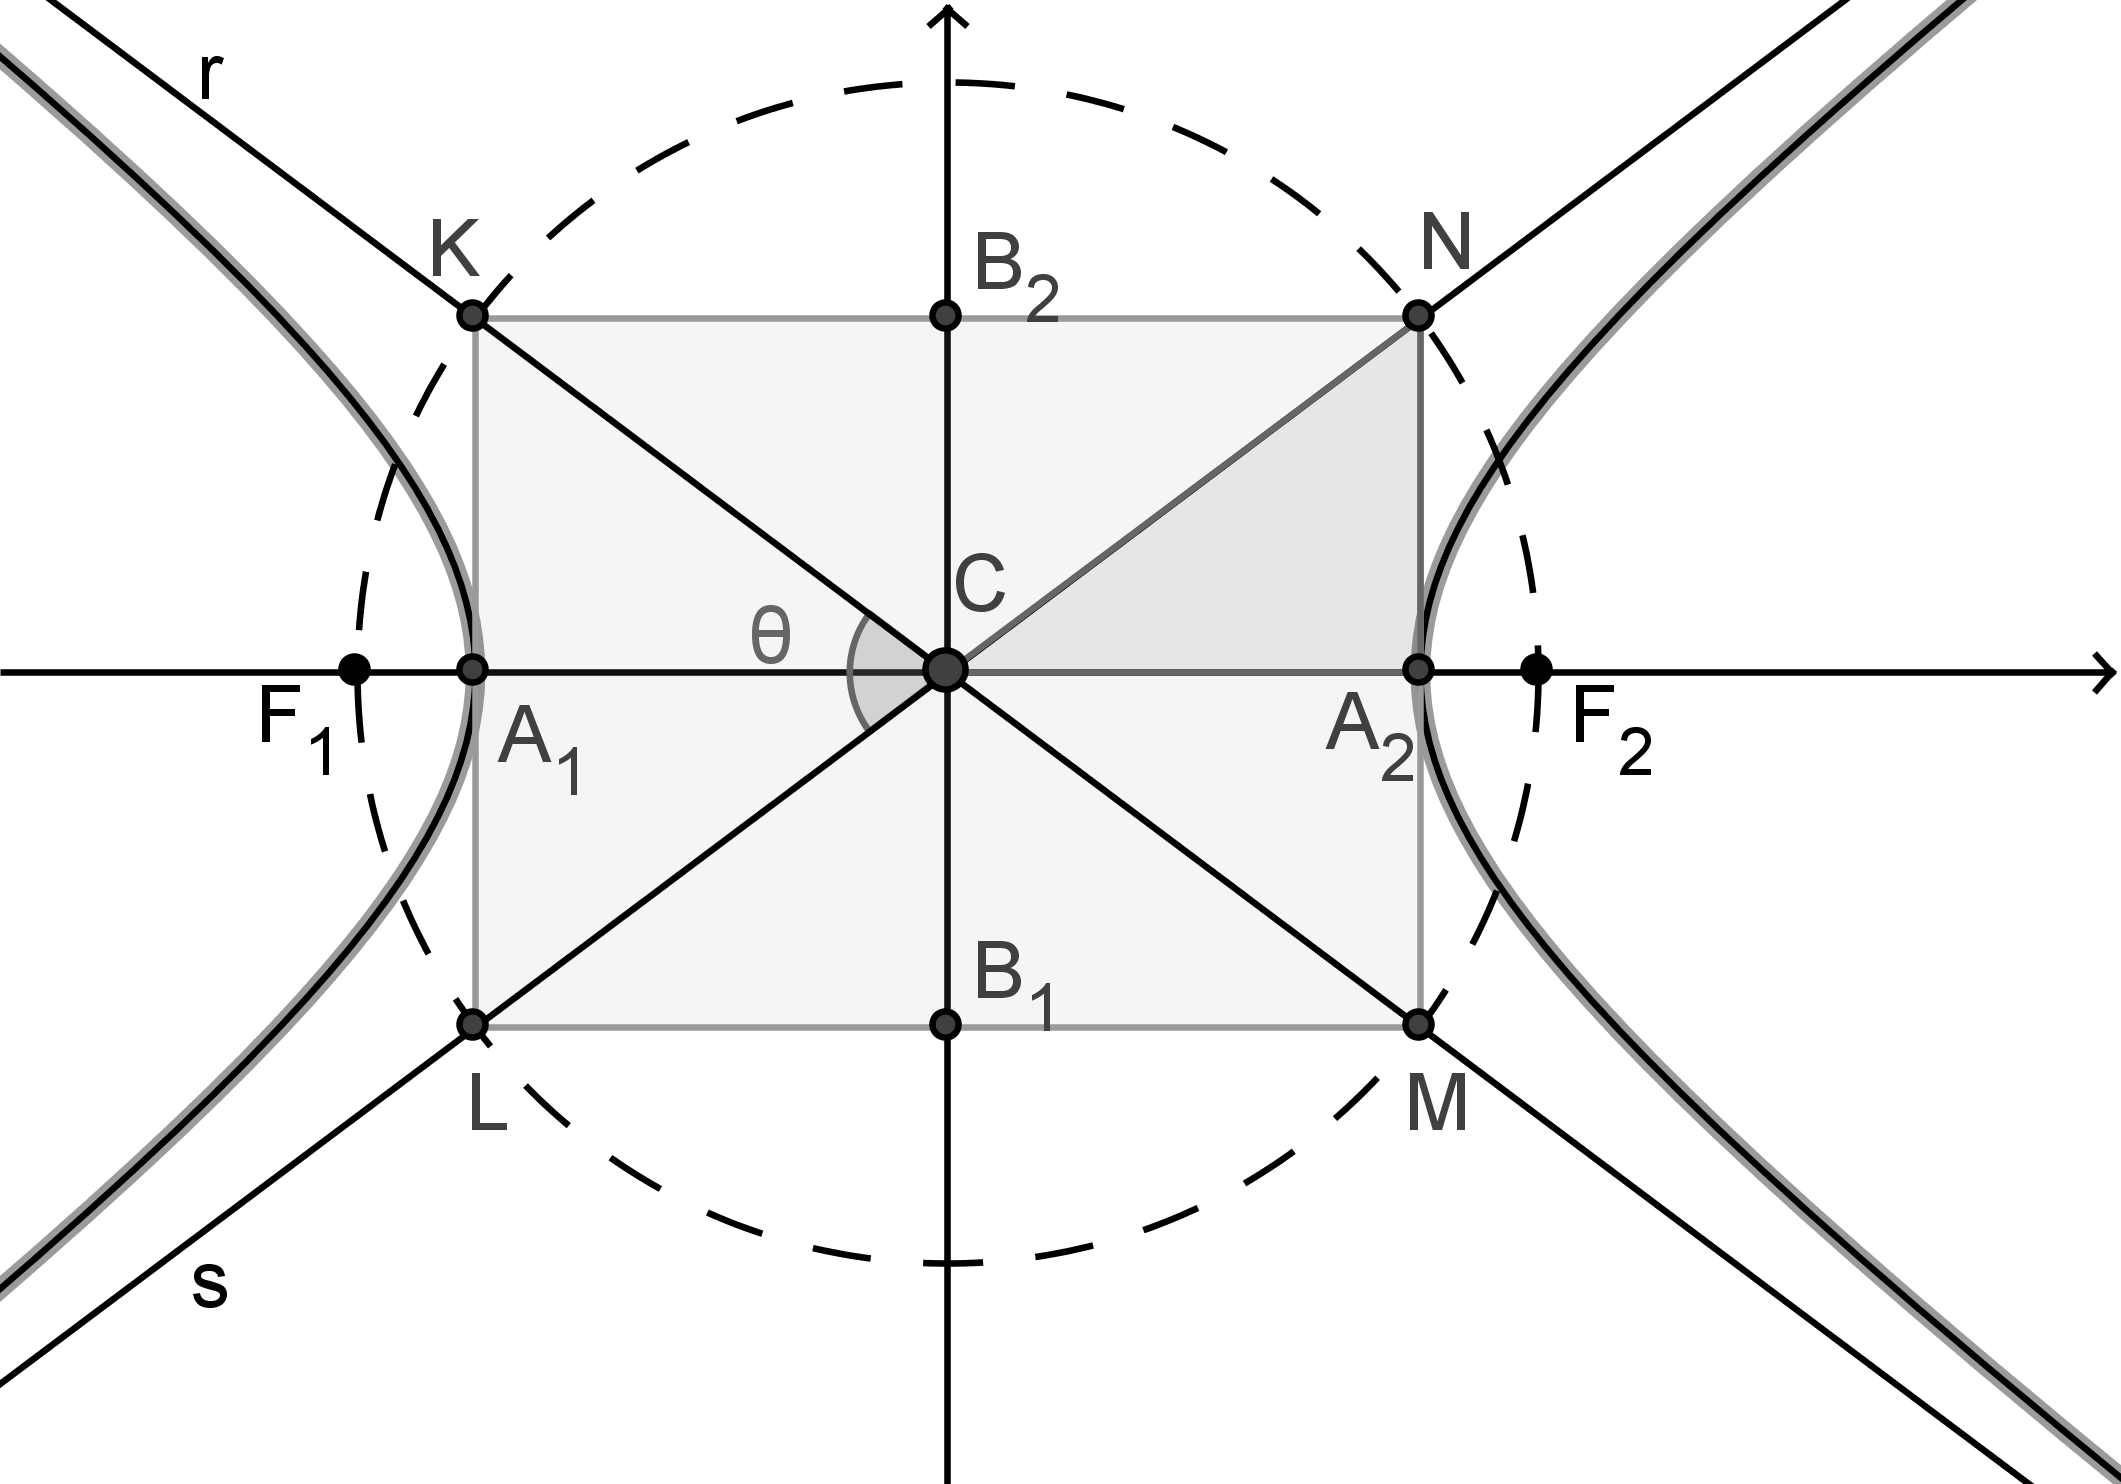
\includegraphics[width=\linewidth]{analitica/imagens/hiperboleh2.png}
\caption{Hipérbole com assíntotas}
\label{fig:hiperbole2}
\end{minipage}
\end{figure}

A hipérbole possui os seguintes elementos:
\begin{itemize}
  \item \textbf{Focos:} são os pontos $F_1$ e $F_2$.
  \item \textbf{Distância focal:} é a distância $2c$ entre os focos.
  \item \textbf{Centro:} é o ponto médio do segmento $F_1F_2$.
  \item \textbf{Eixo real ou transverso:} é o segmento $A_1A_2$ de comprimento $2a$.
  \item \textbf{Eixo imaginário ou não-transverso:} é o segmento $B_1B_2$ de comprimento $2b$. O eixo imaginário é perpendicular ao segmento $A_1A_2$ no centro $C$.
  \item \textbf{Excentricidade:} é o número real $\displaystyle e=\frac{c}{a}$. A excentricidade da hipérbole está relacionada com sua ``abertura'', ou com o ângulo $\theta$ indicado.
\end{itemize}
Observe que: $$c^2=a^2+b^2$$ e esta igualdade mostra que $a$ e $b$ são menores do que $c$.

\subsection{Equações reduzidas da hipérbole}

Considere um sistema cartesiano, e adotemos os focos da hipérbole sobre o eixo $Ox$. Desta forma, use $F_1(-c, 0)$, $F_2(c,0)$, a distância entre os focos $2c$, a constante da definição $2a$ e utilize a fórmula da distância para deduzir a equação reduzida da elipse.
\begin{eqnarray*}
|d(P, F_1)-d(P, F_2)|&=&2a \\
\left| \sqrt{(x+c)^2+y^2} - \sqrt{(x-c)^2+y^2}\right| & = & 2a  \\
&\vdots &\\
\frac{x^2}{a^2}-\frac{y^2}{b^2}& =& 1
\end{eqnarray*}
que é a \textit{equação reduzida} para esta situação.

\begin{figure}[H]
\centering
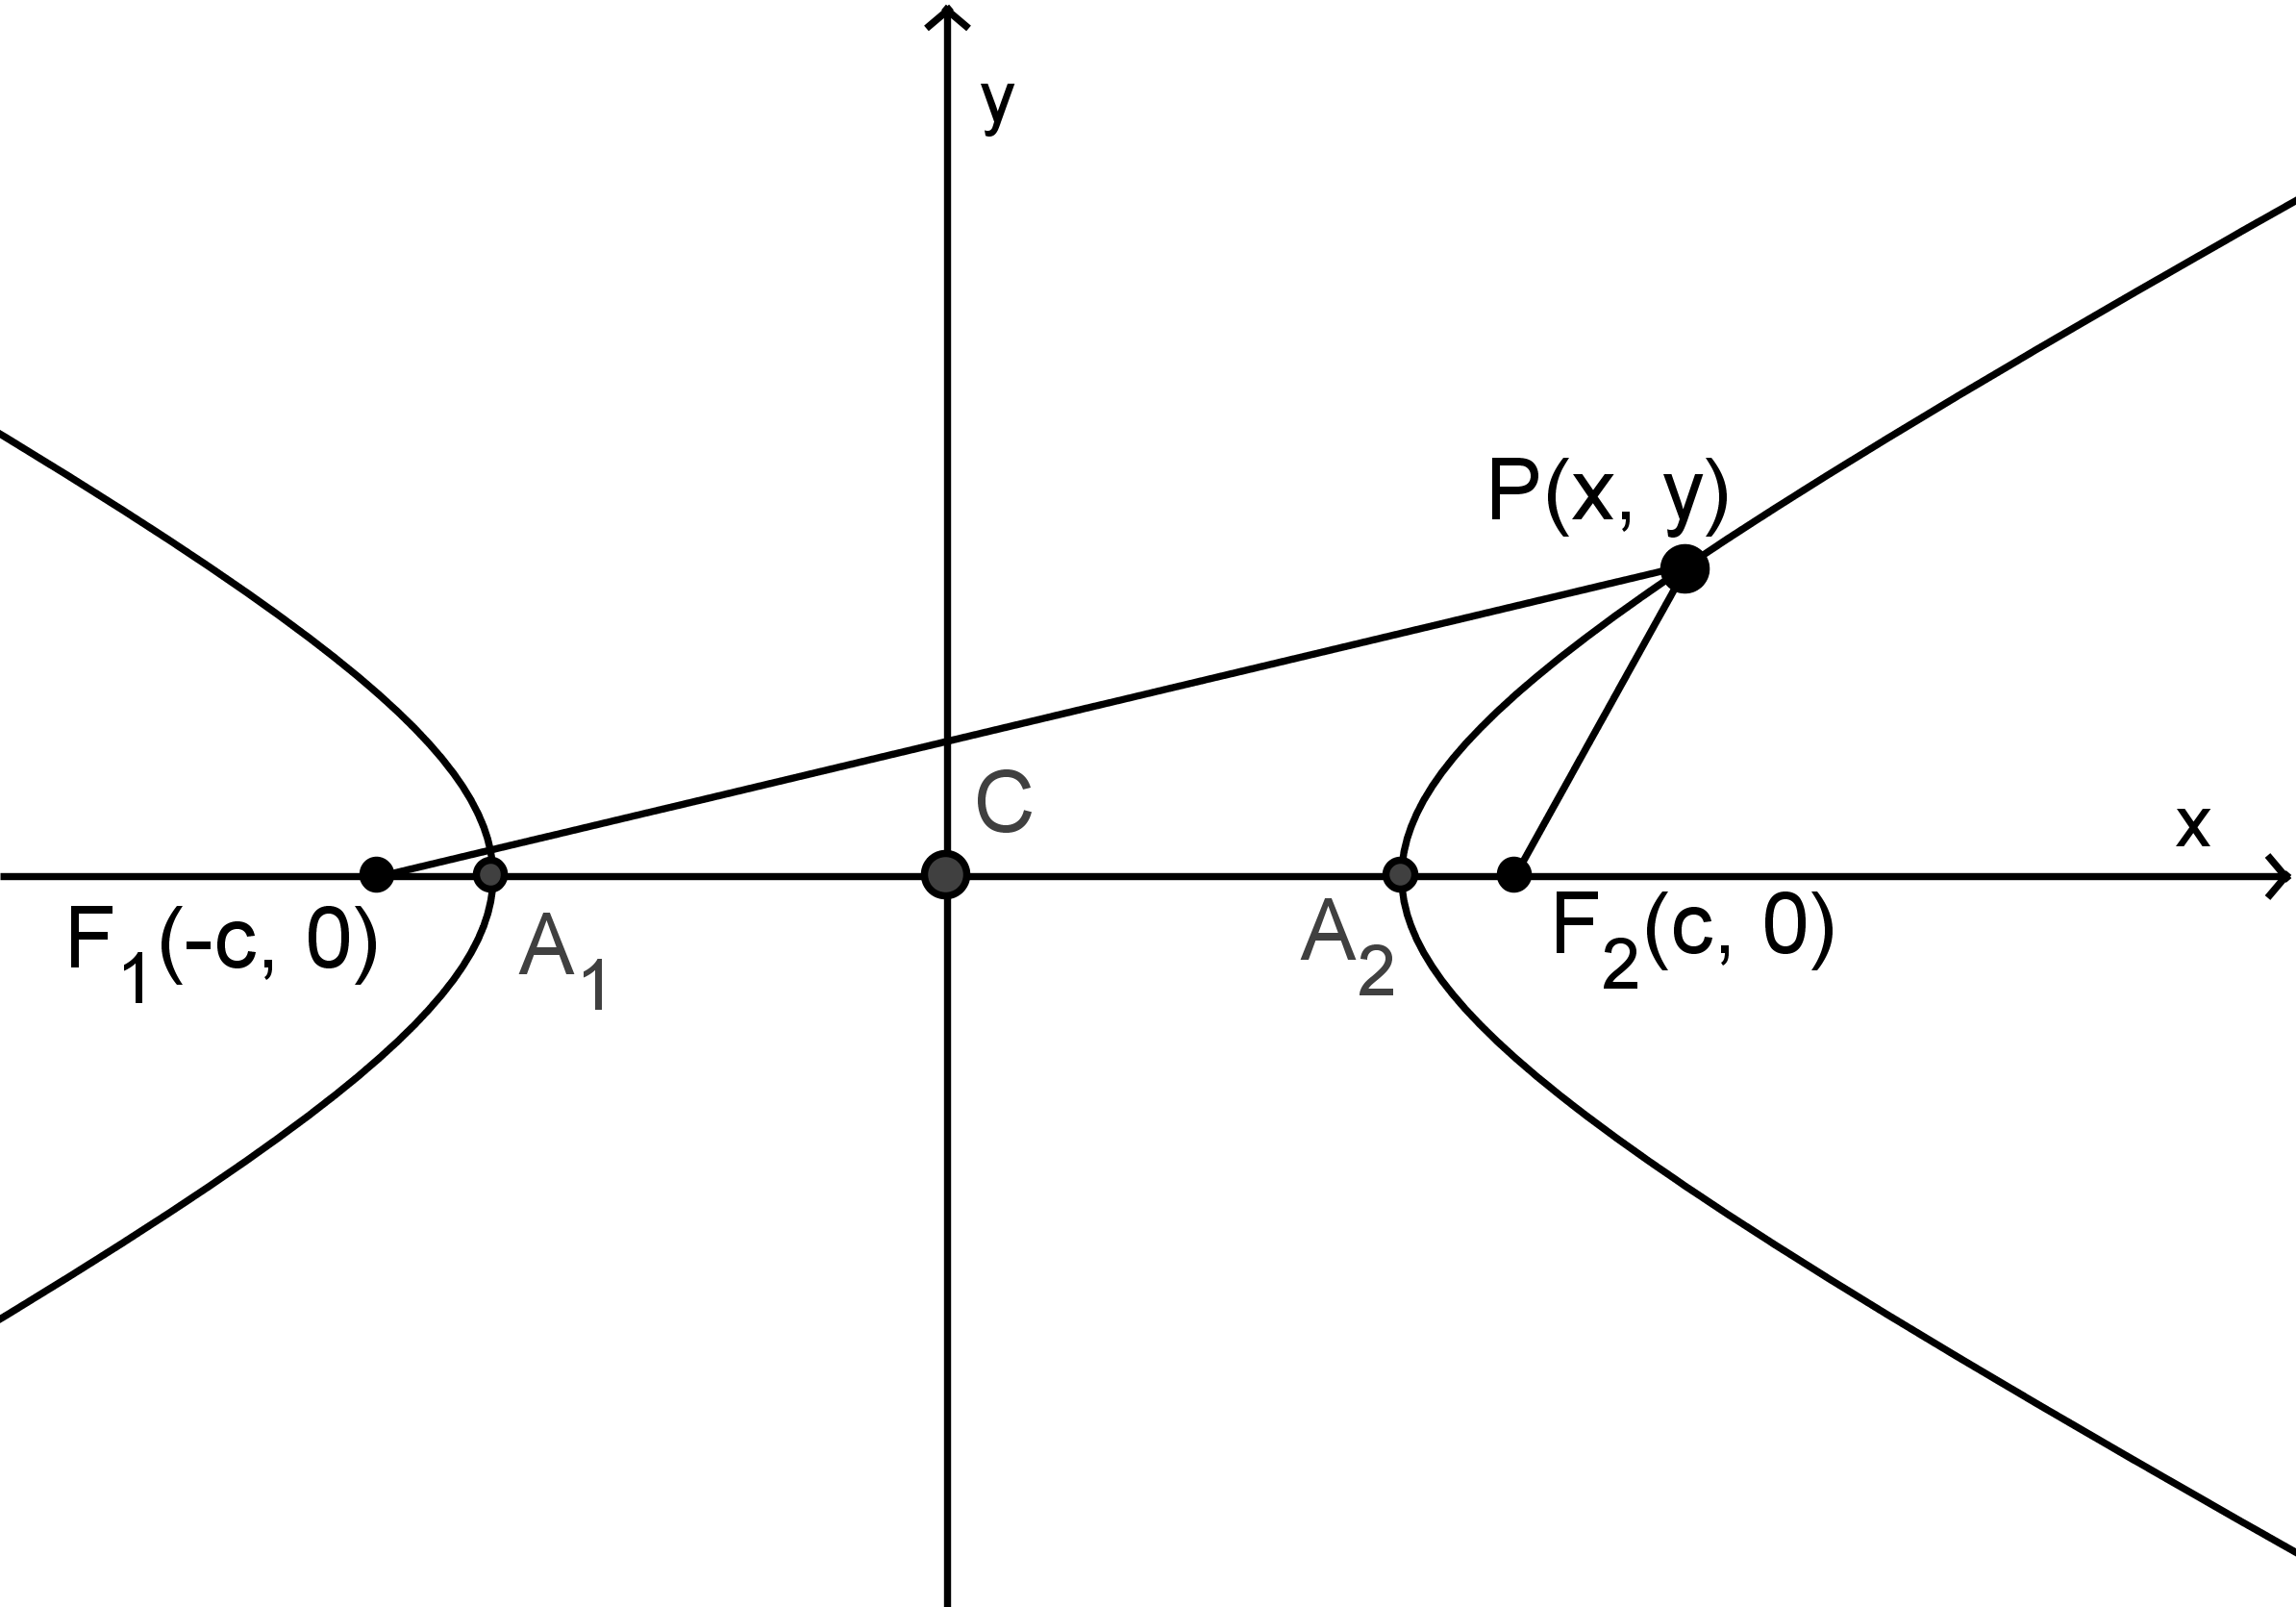
\includegraphics[width=0.45\linewidth]{analitica/imagens/hiperboleh3.png}
\caption{Hipérbole}
\label{fig:hiperh3}
\end{figure}

Para o caso do eixo real sobre o eixo $Oy$, teremos uma situação análoga, com a seguinte \textit{equação reduzida}:

$$\frac{y^2}{a^2}-\frac{x^2}{b^2}=1$$

\begin{figure}[H]
\centering
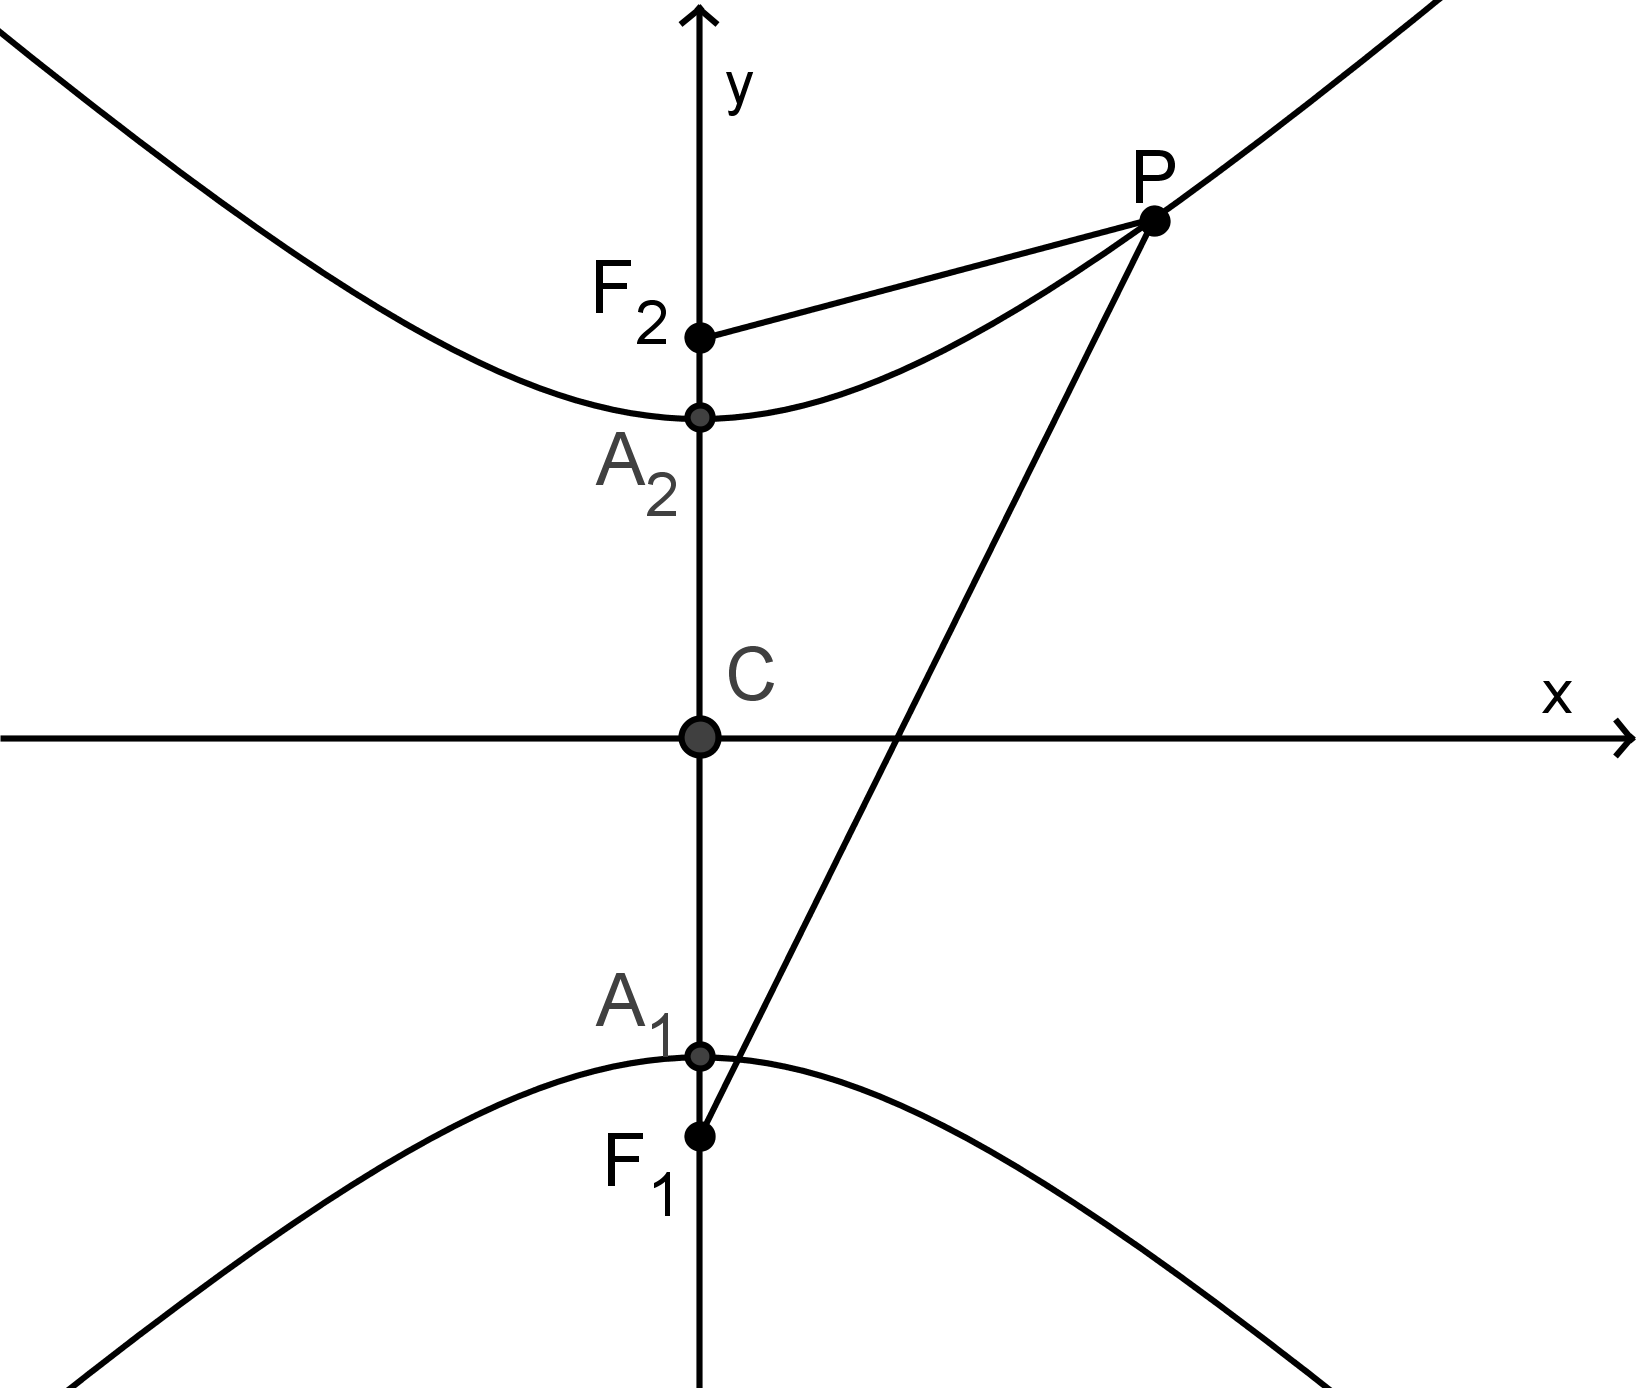
\includegraphics[width=0.35\linewidth]{analitica/imagens/hiperbolev.png}
\caption{Hipérbole com eixo real sobre $Oy$}
\label{fig:hiperv}
\end{figure}

\vspace{1cm}

Para um caso mais geral, considerando o centro da hipérbole em $C(h, k)$, a equação da hipérbole será dada por $$\frac{\left(x-h\right)^2}{a^2}-\frac{\left(y-k\right)^2}{b^2}=1$$ que possui o eixo real paralelo a $Ox$, ou $$\frac{\left(y-k\right)^2}{a^2}-\frac{\left(x-h\right)^2}{b^2}=1$$ que possui eixo real paralelo ao eixo $Oy$.